\chapter{Rivelatori a gas}
\section{Principio di funzionamento}
In un rivelatore a gas \`e formato da una camera piena di materiale gassoso posto tra due elettrodi a diverso potenziale:
quando una particella carica (ionizzante) incide sulla camera, libera coppie di elettroni e ioni; 
queste cariche migrano verso gli elettrodi stabilendo una corrente che \`e proporzionale all'energia deposta nella camera.
Se supponiamo di avere liberato $N$ coppie in seguito alla deposizione di un'energia $E$, allora si pu\`o definire:
\begin{equation*}
W = \frac{E}{N}
\end{equation*}
ovvero l'energia media necessaria per liberare una coppia elettrone-ione.
Questa quantit\`a \`e in genere maggiore dell'energia di legame degli elettroni periferici (25-35 eV), in quanto tiene conto di quell'energia che
viene spesa in eccitazioni atomiche senza ionizzazione.
Gli elettroni prodotti in seguito ad un evento sono in grado di produrre ulteriore ionizzazione, chiamata ionizzazione secondaria, che verr\`a, in
ultima analisi, considerata.\\
Il parametro $W$ \`e un parametro con una blanda dipendenza da tipo di particella e dall'energia deposta,
mentre ha una dipendenza un po' pi\`u pronunciata dal tipo di gas (fig.~\ref{fig:energiaIonizzazioneGas}).
\begin{figure}[htbp]
\begin{center}
	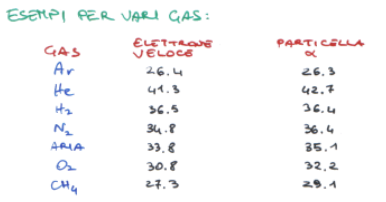
\includegraphics[scale=1]{./Immagini/EnergiaIonizzazioneGas.png}
\caption{Energia di ionizzazione per alcuni gas}
\label{fig:energiaIonizzazioneGas}
\end{center}
\end{figure}
Le fluttuazioni sul numero di coppie prodotte sono di tipo poissoniano:
\begin{equation*}
\sigma_N^2 =F \cdot N
\end{equation*}
con $F$ fattore di Fano, esso \`e minore di 1 nei gas.
\section{Processi all'interno di un rivelatore a gas}
\subsection{Diffusione}
Gli ioni e gli elettroni prodotti all'interno di un gas si diffondono per moto termico; il tipico libero cammino medio per uno ione \`e dai 
$10^{-6}$ ai $10^{-8}$ m.
La diffusione termica degli elettroni \`e di tipo gaussiano con una larghezza che dipende dal tempo secondo la legge:
\begin{equation*}
\sigma = \sqrt{2D\, t}
\end{equation*}
Il coefficiente $D$ di diffusione pu\`o essere determinato nei casi semplici dalla teoria cinetica dei gas, altrimenti tramite modelli di trasporto complessi.
\subsection{Il trasferimento di carica}
Supponiamo di avere due specie X e Y di gas miscelate, quando produco ionizzazione su X posso dar luogo ad una serie di processi detti di trasferimento di carica:
\begin{itemize}
\item L'elettrone che viene liberato viene catturato da Y, di conseguenza ho una coppia (X$^+$, Y$^{-}$)
\item L'atomo ionizzato X$^+$ sottrae carica a un atomo non ionizzato Y, di conseguenza ho una coppia (Y$^{-}$, e$^-$)
\end{itemize}
\subsection{Ricombinazione}
\`E il processo per cui due specie ionizzate X$^-$ e Y$^+$ si neutralizzano formando una specie XY.
Vale la relazione:
\begin{equation*}
\frac{dn^+}{dt} = \frac{dn^-}{dt} = - \alpha \, n^+ \, n^-
\end{equation*}
con $\alpha$ coefficiente di ricombinazione.\\
Esistono due tipi di ricombinazione:
\begin{itemize}
\item \textbf{Ricombinazione colonnare}, avviene immediatamente lungo la traccia della particella ed \`e fortemente dipendente dalla densit\`a di ionizzazione prodotta dalla particella.
Ad esempio le particelle $\alpha$ potranno dar luogo ad un elevata ricombinazione colonnare.
\item \textbf{Ricombinazione volumetrica}, avviene in un secondo momento lontano dalla traccia della particella per la propagazione
delle cariche pi\`u mobili come gli elettroni. Avvenendo dopo un certo tasso di tempo e lontano dalla traccia, la ricombinazione pu\`o avvenire tra ionizzazioni
dovute a tracce differenti, per cui \`e fortemente dipendente dal rate di particelle
\end{itemize}
Per contrastare la ricombinazione volumetrica \`e importante sottoporre il volume ad una differenza di potenziale elevata, in modo da estrarre 
rapidamente ed efficacemente le cariche.
\section{La mobilit\`a e la migrazione delle cariche}
Supponiamo di sottoporre le cariche ad un campo elettrico \textbf{E}, esse migreranno a seconda della carica verso i rispettivi elettrodi.
In generale le collisioni faranno si che esister\`a una velocit\`a media, detta \textbf{velocit\`a di deriva}, tale velocit\`a dipende dal campo
elettrico e dalla pressione secondo la relazione:
\begin{equation*}
v = \mu \frac{\mathbf{E}}{p}
\end{equation*}
con $\mu$ coefficiente di mobilit\`a delle cariche.
Questo coefficiente per gli ioni vale nei $10^{-4}$, portando ad avere diffusioni lente;
per gli elettroni \`e 1000 volte pi\`u  grande (massa 1000 volte pi\`u piccola) portando i tempi per raggiungere gli elettrodi nei $\mu$s.
Il coefficiente \`e costante in ampii range di pressione e campo elettrico per gli ioni, mentre per gli elettroni lo \`e solo per un 
range ristretto di pressione e campo, per via della saturazione.\\
Un'ultima osservazione va fatta per quanto riguarda la diffusione termica: campi pi\`u intensi porteranno ad avere energie e diffusioni maggiori negli elettroni,
per cui si avr\`a una maggiore diffusione in direzione perpendicolare.
Questo non \`e un problema per la raccolta delle cariche, tuttavia disperde gli elettroni (nel mm), facendo perdere risoluzione spaziale.
\section{Le camere a ionizzazione}
\begin{figure}[htbp]
\begin{center}
	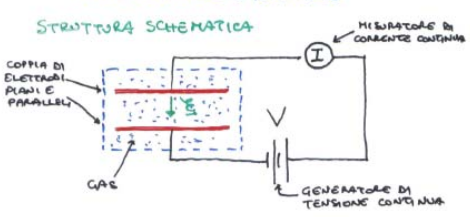
\includegraphics[scale=1]{./Immagini/CameraIonizzazione.png}
\caption{Struttura schematica di una camera a ionizzazione}
\label{fig:cameraIonizzazione}
\end{center}
\end{figure}
\`E un rivelatore che funziona in modalit\`a integrata, in quanto permette di misurare il flusso di radiazione ionizzante.
Supponiamo di avere un flusso di radiazione incidente, esso potr\`a dare luogo ai tre fenomeni: ricombinazione, diffusione fuori dalla camera o verso gli elettrodi;
l'ultimo tipo di evento \`e quello che produce una misura, per contrastare gli altri due \`e necessario aumentare la tensione ai capi della camera.
All'aumentare della tensione si osserva, infatti, un aumento della corrente, fino al raggiungimento di un plateau (fig.~\ref{fig:saturazione}) dovuto alla raccolta completa delle cariche,
in queste condizioni di parla di saturazione del rivelatore e sono le condizioni ottimali di lavoro.
\begin{figure}[htbp]
\begin{center}
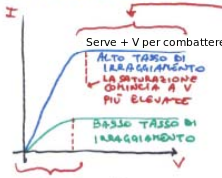
\includegraphics[scale=1]{./Immagini/Saturazione.png}
\caption{Curva tensione-corrente in una camera a ionizzazione, si nota la saturazione}
\label{fig:saturazione}
\end{center}
\end{figure}
Vediamo i fattori che influiscono sulla corrente di saturazione.\\
Il \textbf{tipo di particella} \`e importante, particelle cariche pesanti causano una maggiore ricombinazione colonnare, per cui portano pi\`u in alto il valore
minimo della tensione di saturazione.\\
Un maggiore \textbf{tasso di irraggiamento} implica una maggiore ricombinazione volumetrica, portando in alto la tensione minima.\\
Nel caso vengano usate camere ad aria,\textbf{ l'umidit\`a }\`e un fattore che influisce sulla ricombinazione volumetrica, aumentandola, per questo maggiori umidit\`a
alzano la tensione minima.\\
A causa del moto di deriva delle cariche, lungo gli elettrodi si forma un accumulo di carica che tende a schermarli e a rendere pi\`u difficile la raccolta delle cariche.
Si pu\`o immaginare che si formi un potenziale opposto che genera una corrente di contrasto, \`e possibile trovare la variazione relativa attraverso:
\begin{equation*}
\frac{\Delta I}{I} = \epsilon \frac{k_b T}{e\cdot V}
\end{equation*}
con T temperatura ed $\epsilon$ il rapporto tra l'energia media della particella sotto l'effetto del campo elettrico ed in sua assenza.
Questo rapporto vale circa 1 per gli ioni, ma vale alcune centinaia per gli elettroni.
Per gli elettroni l'energia media raggiunge un plateau all'aumentare della tensione, per questo motivo \`e possibile contrastare questa variazione
di corrente opponendo campi elettrici pi\`u intensi, quindi tensioni maggiori.\\
Per tensioni sufficientemente alte, la ricombinazione volumetrica pu\`o diventare trascurabile, tuttavia questo non accade per la colonnare;
per questo motivo la corrente misurata sar\`a sempre minore della corrente reale di saturazione.
Una stima di quanta corrente si sta perdendo pu\`o essere ottenuto costruendo una curva 1/V - 1/I, interpolandola ed estrapolando il punto a 1/V = 0, ovvero
V infinita (fig~\ref{fig:iPersa}).
\begin{figure}[htbp]
\begin{center}
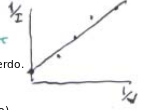
\includegraphics[scale=1]{./Immagini/IPersa.png}
\caption{Stima della corrente di saturazione}
\label{fig:iPersa}
\end{center}
\end{figure}
\section{Funzionamento in modo impulsivo delle camere a ionizzazione}
Il moto delle cariche all'interno della camera induce una corrente ai capi degli elettrodi, questa variazione viene percepita
da un sistema RC che raggiunge una tensione massima quando tutta la carica viene raccolta.
Il tempo caratteristico del circuito determina il tipo di carica raccolta: RC nei $\mu$s saranno sensibili solamente alla raccolta degli elettroni,
RC nei ms saranno sensibili anche alle particelle cariche.
Chiaramente la scelta di RC determina il tasso che il rivelatore \`e in grado di misurare, un RC nei $mu$s sar\`a in grado di rivelare e misurare
a tassi maggiori, tuttavia produrr\`a segnali pi\`u piccoli.
\subsection{Sviluppo del segnale nel tempo}
\begin{figure}[htbp]
\begin{center}
	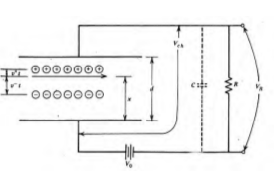
\includegraphics[scale=1]{./Immagini/CircuitoCameraIonizzazione.png}
\end{center}
\end{figure}
Per ottenere lo sviluppo del segnale nel tempo ricorriamo alla conservazione dell'energia, ponendo $V_0$ la tensione iniziale e $V_{ch}$ quella rimanente si ha:
\begin{equation*}
\frac{1}{2} C V_0^2 = n_0 e E v^+ t - n_0 e E v^- t + \frac{1}{2}C V_{ch}^2
\end{equation*}
Portando a sinistra i termini legati al condensatore e dato che $E=-V_{ch}/d$ con $d$ distanza tra gli elettrodi su pu\`o scrivere:
\begin{equation*}
\frac{1}{2} C (V_0+V_{ch})(V_0-V_{ch}) = n_0 e \left(\frac{V_{ch}}{d}\right) t (v^+ - v^-)
\end{equation*}
Dato che $V_{ch}\approx V_0$, $V_0+V_{ch}\approx 2 V_0$ e $V_0 - V_{ch} = V_R$, ovvero la tensione sulla resistenza possiamo scrivere:
\begin{equation}\label{eq:VRCamera}
V_R = \frac{n_0 e (v^+-v^-)}{d\,C}t
\end{equation}
Da cui si pu\`o vedere che la porzione iniziale del segnale ha andamento lineare dipendente dal numero di coppie liberate.
Dalla relazione~\ref{eq:VRCamera} si possono osservare alcune cose:
\begin{itemize}
\item Il moto delle cariche positive ha indotto un potenziale $\frac{n_0 e v^+}{d\,C}t$, lo stesso vale per le negative. 
Questo potenziale pu\`o essere visto come una carica indotta $\frac{n_0 e v^+}{d}t$ ai capi della capacit\`a.
\item Quando la raccolta delle cariche si \`e conclusa $v^- t$ vale $-x$ (\`e opposto al campo) e $v^+ t$ vale $d-x$, per cui si ha:
\begin{equation*}
V_R^{MAX} = \frac{n_0 e}{C}
\end{equation*}
\end{itemize}
\section{Le camere proporzionali}
Supponiamo che una particella da 1 MeV ionizzi il gas contenuto in una camera a ionizzazione, se l'energia media di ionizzazione \`e 35 eV e il condensatore
ha una capacit\`a di 100 pF allora l'ampiezza massima del segnale generato sar\`a:
\begin{equation*}
V_{MAX} = \frac{E\,e}{W \, C} \sim 10 \mu\,\text{V}
\end{equation*}
Il segnale \`e piuttosto piccolo, per questo motivo \`e necessario amplificando cercando di utilizzare la ionizzazione secondaria:
le camere proporzionali si basano su questo principio, le cariche primarie liberate vengono accelerate da un campo che fornisce loro energia sufficiente
a produrre ionizzazione a cascata, come in una sorta di fotomoltiplicatore.
La quantit\`a di ionizzazione prodotta risulta dipendente dalla ionizzazione primaria, quindi dall'energia iniziale della particella, e il segnale
molto pi\`u forte rispetto a quelle prodotto da un rivelatore basato unicamente sulla ionizzazione primaria.\\
Una geometria molto utilizzata in questi rivelatori \`e quella cilindrica: in questi rivelatori il campo elettrico scala come il reciproco del raggio;
per l'aria, se esso supera il valore soglia di $10^6$ V/m allora si possono osservare moltiplicazioni di ionizzazione.
Per un rivelatore dove il campo \`e costante la moltiplicazione \`e esponenziale:
\begin{equation*}
n(x) = n(0) e^{\alpha x}
\end{equation*}
con $x$ spazio percorso e $\alpha$ coefficiente di Townsend.
Questo coefficiente dipende dal campo con l'andamento riportato in figura~\ref{fig:townsend}, per cui per un rivelatore a geometria cilindrica
la moltiplicazione \`e pi\`u che esponenziale.
\begin{figure}[htbp]
\begin{center}
	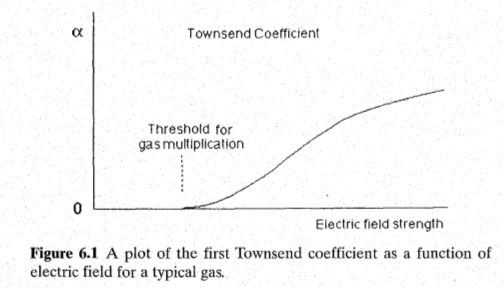
\includegraphics[scale=0.8]{./Immagini/Townsend.png}
\caption{Coefficiente di Townsend}
\label{fig:townsend}
\end{center}
\end{figure}
\subsection{Problemi delle camere proporzionali}
Uno dei problemi fondamentali nelle camere proporzionali sta nella scelta del gas: poich\`e gli elettroni possono ionizzare, eccitare o essere assorbiti a seconda
della molecola con cui interagiscono, la composizione del gas \`e fondamentale.
Ad esempio un gas elettronegativo come l'ossigeno pu\`o essere un problema, per via della sua tendenza ad attrarre elettroni; la presenza di molecole
pu\`o portare ad eccitazioni e diseccitazioni non radiative (mediante stati vibrazionali eccitati).\\
In genere vengono usati gas nobili, come l'Argon, che dissipano l'energia principalmente per ionizzazione; questi, tuttavia, hanno il problema
della diseccitazione, poich\`e essa pu\`o passare unicamente attraverso emissione di fotoni (non ho molecole che si eccitano vibrazionalmente) questi possono
ionizzare gli elettrodi, generando ulteriori scariche a valanga.
Queste scariche possono allungare la durata degli impulsi e il tempo morto del dispositivo, per questo spesso si accompagna questi gas con dei gas
quenchanti che spengono la valanga eccitandosi vibrazionalmente.
Un esempio di gas quenchante \`e il metano che assorbe nella fascia dei 10 eV.
\section{Fluttuazioni statistiche nelle camere proporzionali}
Nelle camere proporzionali abbiamo due principali cause di fluttuazioni statistiche:
\begin{itemize}
\item Fluttuazione nel numero di elettroni primari liberati
\item Fluttuazione nella moltiplicazione del singolo elettrone primario
\end{itemize}
Se supponiamo che le due fluttuazioni siano indipendenti, allora \`e possibile trovare la fluttuazione relativa complessiva sommando gli errori relativi in quadratura;
ponendo $\bar{A}$ la media dei fattori di moltiplicazione di un singolo elettrone si pu\`o scrivere:
\begin{equation*}
\left(\frac{\sigma_{Q}}{Q}\right)^2 = \left(\frac{\sigma_{n_0}}{n_0}\right)^2 +  \left(\frac{\sigma_{\bar{A}}}{\bar{A}}\right)^2
\end{equation*}
La varianza del fattore medio di moltiplicazione vale:
\begin{equation*}
\sigma^2_{\bar{A}} = \frac{\sum_i^{n_0} \sigma^2_A}{n_0^2} = \frac{\sigma^2_A}{n_0}
\end{equation*}
con $\sigma_A$ varianza del fattore di moltiplicazione di singolo elettrone.
Si pu\`o quindi scrivere
\begin{equation*}
\left(\frac{\sigma_{Q}}{Q}\right)^2 = \left(\frac{\sigma_{n_0}}{n_0}\right)^2 + \frac{1}{n_0} \left(\frac{\sigma_{A}}{\bar{A}}\right)^2
\end{equation*}
Il primo termine \`e gi\`a stato trattato nelle camere a ionizzazione, esso vale:
\begin{equation*}
\left(\frac{\sigma_{n_0}}{n_0}\right)^2 = \frac{F}{n_0}
\end{equation*}
Per quanto riguarda il secondo termine, nel caso di bassi campi elettrici \`e possibile ipotizzare che la probabilit\`a di ionizzazione di un elettrone non dipenda dalla sua storia;
se $A>100$ \`e possibile scrivere la probabilit\`a di avere un determinato $A$ al termine di un amplificazione come:
\begin{equation*}
P(A) = \frac{e^{-A}{\bar{A}}}{\bar{A}}
\end{equation*} 
per cui:
\begin{equation*}
\left(\frac{\sigma{A}}{A}\right)^2 = 1
\end{equation*}
Se il campo \`e intenso l'ipotesi di indipendenza dalla storia salta ed \`e necessario considerare un modello pi\`u complesso che porta ad affermare:
\begin{equation*}
\left(\frac{\sigma_A}{A}\right)^2 = \frac{1}{\bar{A}} + b
\end{equation*}
con $b = (1+\theta^2)^{-1}\approx 0.5$ e $\theta$ \`e un parametro che dipende dalla frazione di elettroni con energia superiore a quella di ionizzazione.
\subsection{Sviluppo del segnale}
In una camera proporzionale esistono due tempi caratteristici: il tempo di deriva, che indica il tempo impiegato dagli elettroni a raggiungere la zona
di moltiplicazione (ovvero la regione prossima all'anodo), e il tempo di moltiplicazione, ovvero il tempo impiegato dagli elettroni per effettuare la loro moltiplicazione a cascata.
Il moto delle coppie primarie \`e trascurabile ai fini della forma del segnale, in quanto producono segnali molto piccoli, per questo si pu\`o
dire che i segnali prodotti dalla camera hanno un ritardo nell'ordine del $\mu$s rispetto all'evento, per via del drift delle cariche.
Il tempo di moltiplicazione \`e molto inferiore rispetto a quello di deriva, per cui il tempo di ritardo pu\`o essere assunto pari al tempo di drift.\\
Dato che il segnale viene prodotto vicino all'anodo, il fronte di salita del segnale viene determinato sopratutto dal moto degli ioni positivi:
essi sono immersi in campi intensi che li portano ad avere un'alta velocit\`a di deriva verso il catodo.
Per questo motivo il fronte di salita \`e inizialmente molto veloce, successivamente diventa lento, in quanto gli ioni entrano nella zona a campo debole in cui
sono lenti.\\
Mostriamo che il segnale \`e fortemente dipendente dal moto degli ioni, chiamiamo $E$ l'energia e $\epsilon$ il campo, iniziamo
con il calcolare tempo necessario affinche uno ione raggiunga il catodo.
Si pu\`o approssimare che gli ioni vengano prodotti a ridosso dell'anodo, quindi a raggio $a$, la velocit\`a dello ione vale:
\begin{equation*}
v^+ = \mu \frac{\epsilon}{p} = \frac{\mu}{p} \frac{V_0}{r \, \text{ln}(b/a)}
\end{equation*}
Risolvendo l'equazione differenziale per separazione delle variabili:
\begin{equation*}
v^+(r) = \frac{dr}{dt}
\end{equation*}
si ottiene:
\begin{equation*}
r(t) = \sqrt{2 \frac{\mu}{p} \frac{V_0}{\text{ln}(b/a)} t + a^2}
\end{equation*}
per cui il tempo per raggiungere $b$ vale:
\begin{equation*}
t^+ =\frac{(b^2 - a^2) p \, \text{ln}(b/a)}{2 \mu V_0}
\end{equation*}
Inserendo dati tipici si ottiene che questo tempo vale nelle centinaia di $\mu$s;
studiando l'andamento temporale dell'energia si ottiene, tuttavia, che la maggior parte del segnale si sviluppa in breve tempo:
\begin{equation*}
\frac{1}{2} C \, V_0^2 - \frac{1}{2} C \, V_{ch}^2 = \Delta E
\end{equation*}
in modo simile a quanto fatto prima, si trova che $V_R = V_0 - V_{ch}$ vale:
\begin{equation*}
V_R(t) = \frac{\Delta E(t)}{C V_0}
\end{equation*}
Calcoliamo $\Delta E(t)$:
\begin{equation*}
\frac{dE}{dx} = Q \epsilon = Q \frac{V_0}{r \, \text{ln}(b/a)}
\end{equation*}
per cui:
\begin{equation*}
\Delta E(t) = \frac{Q \, V_0}{ \, \text{ln}(b/a)} \int_a^{r(t)} \frac{1}{r} \, dr  =  \frac{Q \,V_0}{ \text{ln}(b/a)} \text{ln}\left(\frac{r(t)}{a}\right)
\end{equation*}
Usando $r(t)$ trovato predecentemente si trova:
\begin{equation*}
V_R(t) =\frac{ \Delta E(t)}{C \, V_0} = \frac{Q}{C} \frac{1}{\text{ln}(b/a)} \text{ln} \left(\frac{2\mu V_0}{a^2 p \text{ln}(b/a)}t+1\right)^{\frac{1}{2}}
\end{equation*}
Il tempo affinche si raggiunga mezza ampiezza vale:
\begin{equation*}
t = \frac{a}{a+b} t^+
\end{equation*}
ed \`e nei $\mu$s.\\
Questi conti sono validi nell'ipotesi di elettroni moltiplicati in un punto fisso, altrimenti si osserva uno spreading dei tempi.\\
Tipicamente i tempi del RC non sono tali da permettere una raccolta completa delle cariche, per questo si ha il problema del deficit balistico.
Infine gli elettroni contribuiscono nel \% all'ampiezza del segnale, in quanto percorrono poco spazio nella camera.
\section{Contatori Geiger-M\"uller}
\begin{figure}[htbp]
\begin{center}
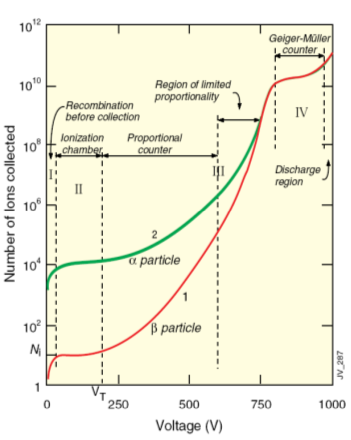
\includegraphics[scale=1]{./Immagini/RegioniGas.png}
\caption{Regioni di lavoro di un rivelatore a gas}
\label{fig:regioniGas}
\end{center}
\end{figure}
Aumentando la tensione ai capi di una camera a gas si pu\`o aumentare ulteriormente la moltiplicazione degli elettroni, in particolare si pu\`o raggiungere
una regione detta di saturazione, dove si satura la camera e ogni evento produce la medesima ionizzazione.
Questa regione \`e quella in cui operano i rivelatori di Geiger-M\"uller: questi dispositivi producono impulsi medesimi indipendentemente dalla ionizzazione
iniziale (quindi dall'energia).
Questi rivelatori non sono, quindi, adatti per misure di spettroscopia, tuttavia possono essere utilizzati come contatori a bassi rate.
L'elevato fattore moltiplicativo dei contatori Geiger ($\sim 10^{10}$) produce segnali nei volt che possono essere usati per alimentare un altoparlante, da qui
il click tipico di questi dispositivi.
La cascata in questi dispositivi \`e fortemente determinata dalla diseccitazioni dei gas, infatti esse producono fotoni nell'ultravioletto in grado
di produrre scariche secondarie in regioni remote del gas (dato che ha bassa probabilit\`a di assorbire il fotone) generando ulteriori
valanghe e fotoni UV (fig.~\ref{fig:valangaGM}).
Per questo motivo nei GM non \`e possibile determinare il punto di interazione della particella incidente.
\begin{figure}[htbp]
\begin{center}
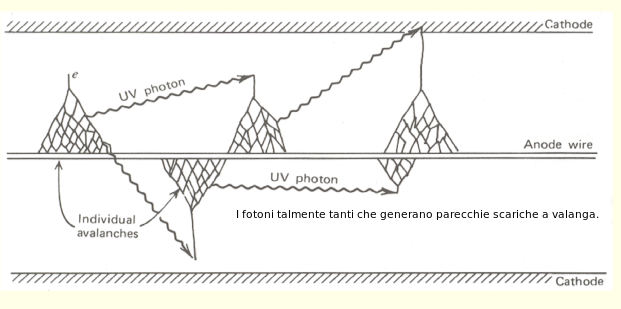
\includegraphics[scale=0.7]{./Immagini/ValangaGM.png}
\caption{Scarica in un contatore GM}
\label{fig:valangaGM}
\end{center}
\end{figure}
Il gas usato nei rivelatori \`e spesso un gas nobile, ma \`e possibile utilizzare anche l'aria.\\
La scarica prodotta nei GM \`e talmente violenta che \`e necessario introdurre dei meccanismi di spegnimento della moltiplicazione,
spesso si procede con un interruzione dell'alimentazione dopo un certo tempo. 
Questa interruzione porta ad avere tempi morti piuttosto elevati, per questo i GM non possono essere utilizzati in caso di alti rate di interazione.\\
Per quanto concerne i segnali, i fronti di salita dei GM sono pi\`u lenti di quelli delle camere proporzionali, per via delle valanghe lontane,
in genere sono nei $\mu$s. 
I fronti di discesa sono molto pi\`u lenti, si usano formature con tempi inferiori a 100 $\mu$s.
Il tempo morto in questi dispositivi \`e nei 100 $\mu$s, in quanto \`e necessario assicurarsi che non siano presenti ulteriori scariche libere
che possano generare scariche all'accensione del campo elettrico.
Inoltre le cariche positive libere riducono il campo elettrico, impedendo la formazione di nuove cascate, influendo sul tempo morto.